    %One way to view the structure of conversations is as a long string of adjacent \glspl{da}. Tagging these \glspl{da} automatically is an active area of research, because it helps speech controlled devices (such as Google Home or Amazon Alexa) identify what the user wants. All state of the art methods (see Sec. \ref{ssec: da classification}) use \glspl{rnn} for this task.

    %\gls{da} classification is an active area of research, because it helps speech controlled devices (such as Google Home or Amazon Alexa) identify what the user wants\cite{daApplications}. We select an existing hierarchical bi-directional \gls{lstm} \gls{model} by Kumar et al.\cite{kumar2017dialogue} (for the reasons explained in Sec. \ref{sssec: kumar model}) and modernise it.

    \section{Training Data}
    To train \glspl{nn}, a set of training data of \glspl{utterance} $\mathcal{U}$ with their correctly labelled \glspl{da} $\mathcal{D}$ is required. The two datasets that are commonly used in the literature are the \gls{swda} corpus\cite{swda} (see Sec. \ref{ssec: swda}) and the Meeting Recorder Dialogue Dct (MRDa) corpus\cite{shriberg2004icsi}. We limit ourselves to the \gls{swda} corpus, because we believe the style of conversations in the \gls{swda} corpus to more closely resemble \textit{natural} conversations than the meeting transcriptions in the MRDA corpus. We are, however, confident that our improvements generalise well to the MRDA corpus.

    \section{Initial Model \label{method: kumar model}}
    
    \begin{table}
    \centering
        \begin{tabular}{|l|l|}
        \hline
        \textbf{Hyperparameter}      & \textbf{Value} \\ \hline
        Nr of Consecutive RNN Layers & 1              \\ \hline
        Nr of RNN Neurons per Layer  & 300            \\ \hline
        Learning Rate $\alpha$       & 1.0            \\ \hline
        Dropout Rate\footnotemark                 & 0.2            \\ \hline
        Loss Function $\mathcal{L}$  & CRF-loss\cite{originalCRF} \\ \hline
        \end{tabular}
        \caption{\label{table: da hyperparams} The hyperparameters used in the initial model. }
    \end{table}
    The \gls{model} proposed by IBM Research in \cite{kumar2017dialogue} is a hierarchical Bi-LSTM-CRF \gls{model}, which first encodes \glspl{utterance} using an \gls{embedding} and \gls{lstm} layer and then uses these encoded \glspl{utterance} in a combination with another \gls{lstm} layer and a \gls{crf} layer to classify the \gls{da} of every \gls{utterance}. The entire \gls{model} architecture is displayed in Fig. \ref{fig:kumar_model}. The exact specifications of the model, the hyperparamters, are shown in Table \ref{table: da hyperparams}. 
    
    \footnotetext{The \textit{dropout rate} is a parameter of \gls{rnn} \glspl{neuron} --- during training, with probability equal to the dropout rate, a \gls{neuron} does not fire even though it should. Dropout makes the training process more robust and is disabled in actual predictions\cite{mlTextbook}.}

    \begin{figure}
        \centering
        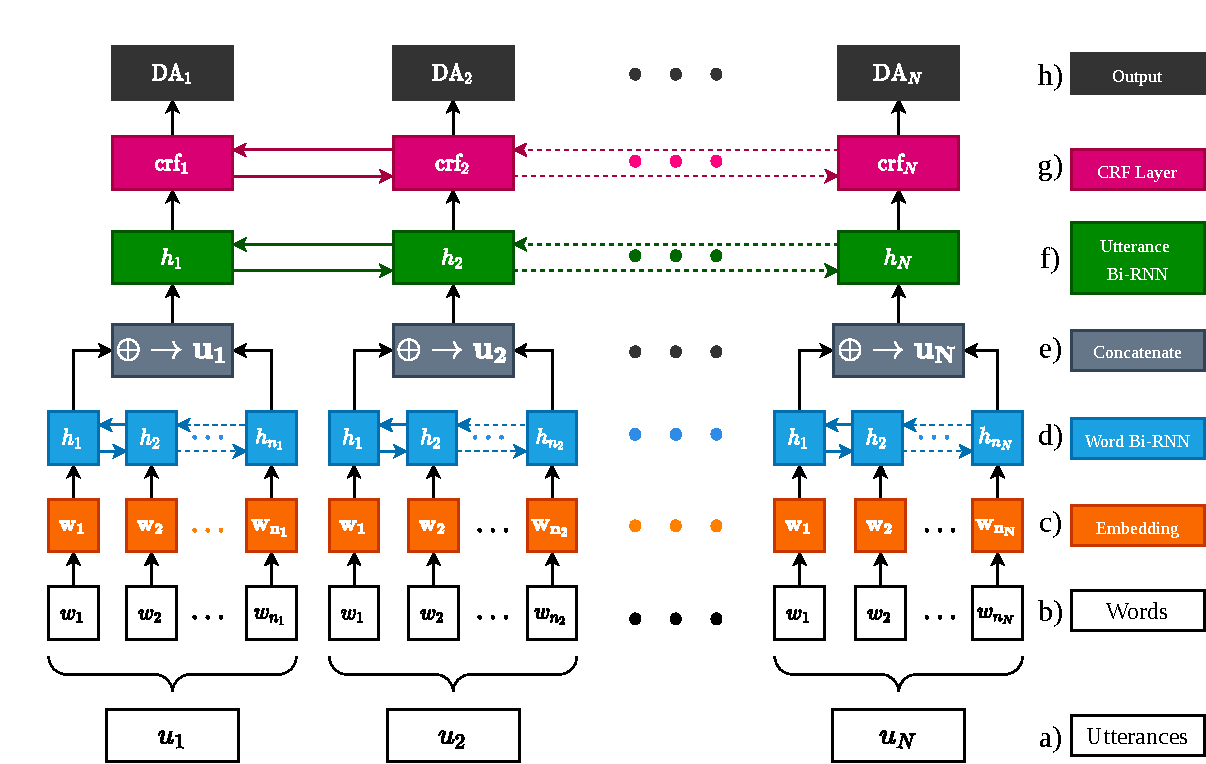
\includegraphics[width=\textwidth]{kumar.pdf}
        \caption{a) $N$ \glspl{utterance} $u_i$ are input into the \gls{model}. \newline 
        b) \Glspl{utterance} are split into lists of words $w_j$. \newline 
        c) $w_j$ are individually embedded into word-\glspl{embedding} $\mathbf{w_j}$ (see Sec. \ref{ssec: word embeddings}).\newline 
        d) The first Bi-\gls{rnn} layer (on the word level) combines all $\mathbf{w_j}$ within $u_i$ into two vectors of numbers, one for the ``forward" direction and one for the ``backward" direction of the \gls{rnn} (see Sec. \ref{ssec: bidirectional RNN}).\newline 
        e) These vectors are concatenated into one vector $\mathbf{u_i}$ that can be understood as the \gls{embedding} of the \gls{utterance} $u_i$.\newline 
        f) \Gls{utterance} \glspl{embedding} $\mathbf{u_i}$ \glspl{embedding} are again combined using a bi-directional \gls{rnn} layer, but this time not just the two final states of the ``forward" and ``backward" direction are passed on, but all hidden states $h_i$ are (see Sec. \ref{ssec: outputting hidden states}).\newline 
        g)A \gls{crf} layer (see Sec. \ref{fig: HMM and CRF}) makes the final classification, which is the sequence of \glspl{da} $\text{DA}_i$ associated with \glspl{utterance} $u_i$ shown in h).}
        \label{fig:kumar_model}
    \end{figure}

    \section{New Implementation}
        The code made public by the researchers is unfortunately not functional and as it is written in an outdated framework (TensorFlow 1.3.0\cite{tensorflow2015-whitepaper}) for python, we were unable to fix the bugs. We therefore re-implement the \gls{model}, with the same hyperparameters, in the more modern Keras library\cite{chollet2015keras} which is a high-level library that makes the low-level TensorFlow 2.3.0 library more easily accessible. Our code is published on ??? (can not include name!).

    \section{Memory Problems}
        Due to limited resources, we ran the training and prediction process on a personal computer on a single NVIDIA GTX 1660Ti graphics card. This graphics card only has 6GB of internal memory, and because the \gls{model} needs to be able to handle conversations of up to 3000 sentences each up to 150 words of length, the storage used by the number of parameters of the \gls{model} far exceeds these 6GB ($\approx$25GB are required). We fix this issue by making the following assumption: The context of sentences matter, but only to an extent. It is unlikely that a \gls{da} of a sentence spoken 100 sentences ago, $d_{i}$ ago impacts the \gls{da} classification of  $d_{i + 100}$. Thus we split the text into chunks of 100 sentences, classify these chunks and re-assemble them.

        \subsubsection{Boundary Effects}
            The chunking process leads to unwanted boundary effects: at the boundary of each chunk, the \gls{model} loses the previous (or following) sentence's information. The context is lost. To mitigate this, we introduce a novel method of recombining chunks. We don't only classify a chunk, say $u_{i}$ to $u_{i + 100}$, we also classify an offset chunk, say $u_{i + 50}$ to $u_{i + 150}$. We then recombine the classified chunks in a way that ensures that no \textbf{final} classification was made near a false boundary. The process is illustrated in Fig. \ref{fig:chunking process}. Given that we obtain the same accuracy as reported in the original paper\cite{kumar2017dialogue} using this method, it is clear that our assumption holds and this method does not significantly diminish the \gls{model}'s accuracy.

    \begin{figure}
        \centering
        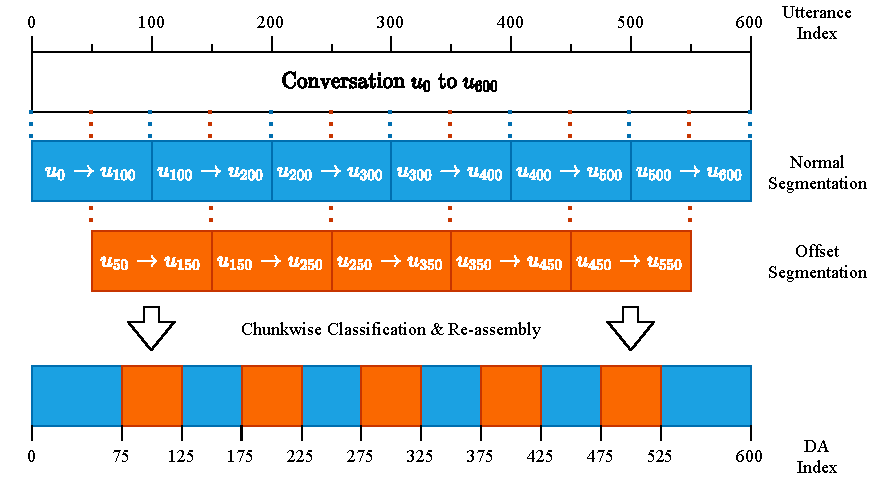
\includegraphics[width=\textwidth]{figures/chunks.pdf}
        \caption{The \glspl{utterance} are split into chunks of 100 twice: once starting at 0 (blue) and once offset, starting at 50 (orange). We classify each chunk independently and overlay them for the final classification so that each of the final \glspl{da} was classified as far from an artificial boundary as possible to minimise context information loss at boundaries.}
        \label{fig:chunking process}
    \end{figure}

    \section{Fixing Tokenisation Bug \label{sec: method tokenisation bug}}
        After we re-implemented the \gls{model}, we achieve the accuracy of $79.2\% \pm 0.3\%$ that is reported by Kumar et al.\cite{kumar2017dialogue}
        However, we found a bug in the implementation which leads to some missed words and to some ends of sentences to be wrongly discarded: To embed an \gls{utterance}, it must first be split into its constituent words. Kumar et al. split the text on whitespace only, which leads to trailing punctation. For example, the sentence
        \begin{equation*}
            \text{Is that house's roof green?}
        \end{equation*}
        is split into the following tokens:
        \begin{equation*}
            \text{[Is, that, \color{red} house's, \color{black} roof, \color{red} green? \color{black}]}.
        \end{equation*}
        The red tokens are not recognised as words within the pre-trained \glspl{embedding} and their information is therefore lost. We fix this bug by splitting the same sentence in the following way:
        \begin{equation*}
            \text{[Is, that, house, ', s, roof, green, ?]}
        \end{equation*}
        The punctuation, as well as the single ``s" have their own \glspl{embedding} which leads to two improvements:
        \begin{enumerate}
            \item Words are no longer made invalid by the punctuation.
            \item The information that the punctuation itself carries is now propagated to the \gls{model}.
        \end{enumerate}
        This change increases the \gls{model}'s accuracy to $81.0\% \pm 0.3\%$.



    \section{Changing Embeddings}
    We change the \glspl{embedding} from \gls{glove} \glspl{embedding} used by Kumar et al.\cite{kumar2017dialogue} to the more sophisticated \gls{numberbatch} \glspl{embedding} (see Sec. \ref{fig: conceptnet}). We also allow the \gls{model} to change the \glspl{embedding} (via training) which optimises these general purpose \glspl{embedding} within this specific context of \gls{da} classification.

    \subsection{Modernising RNN cells}
    Kumar et al.\cite{kumar2017dialogue} use \gls{lstm} cells (see Sec. \ref{ssec: rnn architectures}) as the components of their \gls{rnn} layers. We instead use the more modern \gls{gru}\cite{chung2014empirical} \glspl{neuron} (see Sec. \ref{ssec: rnn architectures}), which require less time to train and are less prone to overfitting (an issue of \gls{ml} models, in which the \gls{model} is too sensitive and understands random noise in the training data as a pattern leading to worse performance on unseen data)\cite{chung2014empirical}.

    \section{Evaluation \label{ssec: method my da model evaluation}}
    
    \begin{figure}[t!]
        \centering
        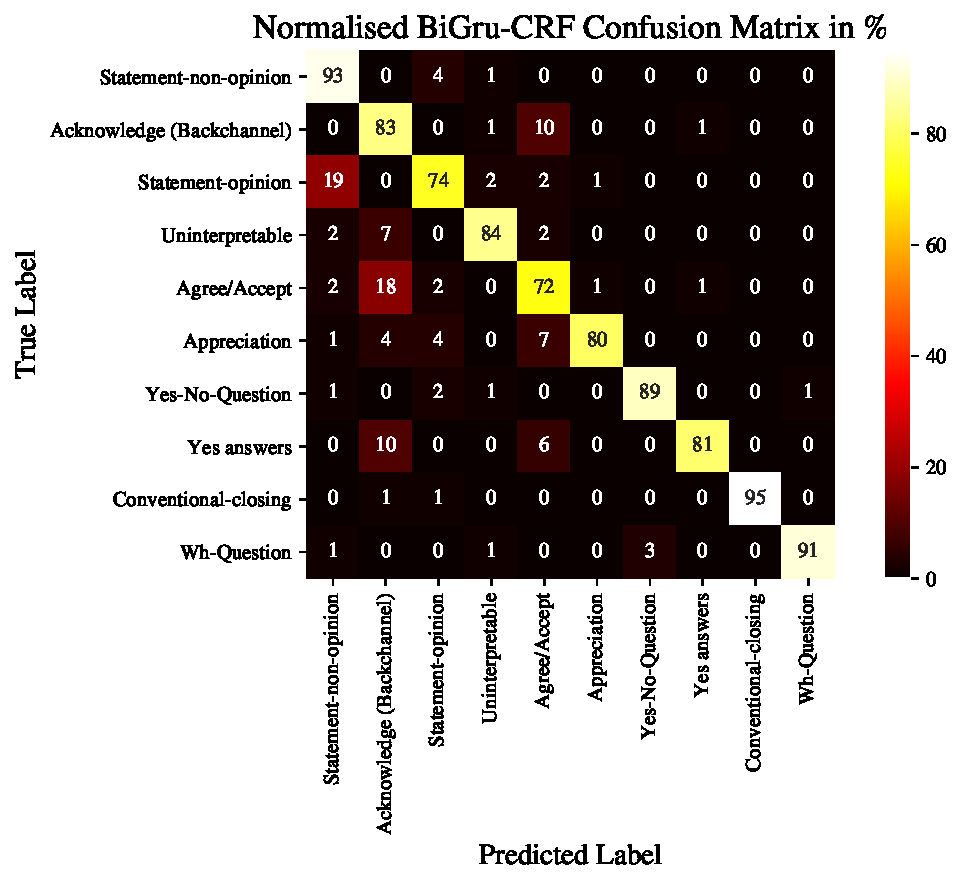
\includegraphics[width=\textwidth]{confusion_gru.pdf}
        \caption{The confusion matrix of our final \gls{da} classifier showing the 10 most frequent \glspl{da}. The field in row $i$ with label $d_i$ and column $j$ with label $d_j$ shows the percentage of \glspl{utterance} with true labels $d_i$ being classified as label $d_j$. The diagonal entries represent the percentage of correctly labelled \glspl{utterance}. Uncertainties are of order $0.1\%$ (varying across \gls{da} categories based on frequencies within the test data) and are excluded for clarity. Because we limit the matrix to the 10 most frequent \glspl{da} (and because we round), rows don't sum to 100\%.}
        \label{fig:confusion}
    \end{figure}
    
    \glsreset{swda}
    To evaluate our final \gls{model}, we randomly split the \gls{swda} corpus into 90\% training data and 10\% test data. The \gls{model} is trained only on the training data and only evaluated on the test data as is standard practice when evaluating any \gls{ml} \gls{model}\cite{mlTextbook}. This process ensures that the \gls{model} has not seen the evaluation data (simulating the real application of the \gls{model}) leading to an unbiased accuracy measurement.
    Our final \gls{model}, which is the \gls{model} introduced by Kumar et al.\cite{kumar2017dialogue} with a fixed bug, using improved word \glspl{embedding}, and more modern \gls{rnn} components outperforms the original \gls{model} so significantly that it is currently the state of the art \gls{da} classification \gls{model}, achieving an accuracy of
    \begin{equation}
        \text{accuracy} = 84.6 \% \pm 0.3\%,
        \label{eq: my da model accuracy}
    \end{equation}
    showing a greater accuracy than the (much more complex) previous state of the art \gls{model} by Ravi et al. at 83.1\%\cite{ravi2018self}. Perhaps more significantly, the humans that originally annotated the \gls{swda} corpus only had 84\% agreement\cite{swda}--- meaning that this \gls{model} is as good as (if not slightly better than) individual humans at labelling \glspl{da}. 
    
    The complete confusion matrix, detailing the model's accuracy for every \gls{da}-type (and its mis-classifications) is shown in Fig. \ref{fig:confusion}. From it, we can identify remaining weaknesses. For example, in $19\%$ of cases, the model confuses \glspl{da} \textit{Statement-opinion} as \textit{Statement-non-opinion}, which can be explained by the difficulty in determining whether a speaker presents a fact or is just speaking with conviction (a mistake that humans can also make). Similarly, it confuses \textit{Agreements}, \textit{Acknowledgements}, \textit{Yes answers} and \textit{Appreciations}. Overall, there is no category in which our classifier performs unexpectedly poorly. We specifically draw attention to the $89 \%$ accuracy in \textit{Yes-No-Questions questions} and $91\%$ accuracy in \textit{Wh-Questions}, which significantly out-performs the original model at $79.8\%$ and $78.2\%$ respectively\cite{kumar2017dialogue}. We believe this discrepancy to be due to the tokenisation bug described in Sec. \ref{sec: method tokenisation bug}, which deletes the information carried by question marks. \newline
